\documentclass{article}
\usepackage[utf8]{inputenc}
\usepackage[T5]{fontenc}
\usepackage{graphicx}
\usepackage[margin=2cm]{geometry}
\title{Report 9: Histogram Equalization}
\author{Nguyễn Thanh Hùng -- 2540056}
\date{}

\begin{document}
\maketitle

\section{Implementation}
I used atomic additions to count 256 grayscale histogram bins. The histogram is reset before each measured run. On the CPU, I calculated a CDF lookup table; a $16\times16$ CUDA kernel applies it to the image. Constant images are preserved. I checked the histogram and output against NumPy.

I ran the notebook on Google Colab with a Tesla T4 and a $256\times256$ sample image.
GPU timings use \texttt{time.time()} after warm-up and synchronization, averaged over three runs; allocation and image transfers are excluded. Where measured, CPU time is one run; speedup is relative to that Python CPU implementation.

\section{Results}
\begin{center}
\begin{tabular}{lr}
\hline
Operation & GPU (ms) \\
\hline
Histogram & 0.1205 \\
Equalization map & 0.0927 \\
\hline
\end{tabular}
\end{center}
Histogram count: 65536 pixels, equal to $256\times256$. Maximum output error: 0. CDF construction is performed on the CPU and is not included in the kernel times.
\begin{center}
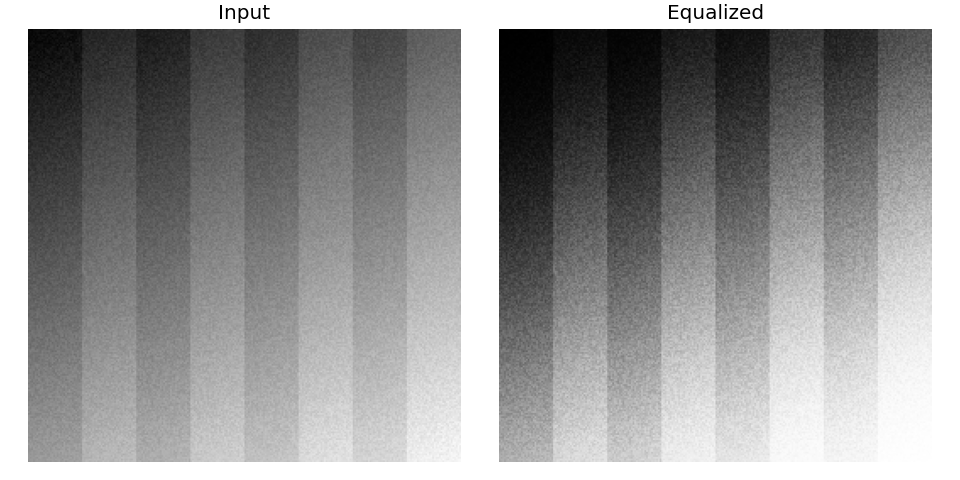
\includegraphics[width=.85\linewidth,height=.19\textheight,keepaspectratio]{figures/images.png}
\end{center}
\begin{center}
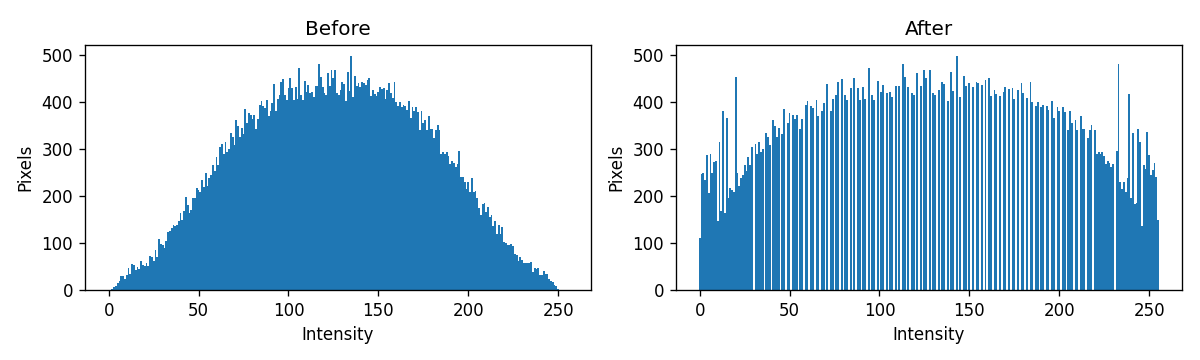
\includegraphics[width=.85\linewidth,height=.18\textheight,keepaspectratio]{figures/histograms.png}
\end{center}

\section{Discussion}
The histogram and mapped output matched the NumPy reference. The before/after histograms show how equalization redistributes grayscale intensities.

\end{document}
